\chapter[Resultados Alcançados]{Resultados Alcançados}


\section{Teste de Viabilidade do Tema}

	Para testar a viabilidade do tema proposto, a ideia foi criar um programa constituído por objetos que fossem fáceis de variar o número de polígonos. Esses objetos escolhidos foram esferas pela facilidade de implementação, pois já existe uma função pronta da biblioteca \textit{glut} chamada \textit{glutSolidSphere}, no qual se cria uma esfera baseada no tamanho do raio, número de cortes latitudinais e longitudinais. O número total de polígonos se dá pela multiplicação destes dois últimos parâmetros como é mostrado em \cite{poly}.  Além disso, estas esferas possuem diferentes movimentações, em que garante-se a ocorrência de oclusão entre elas e diferentes distâncias com relação à câmera. Feito isto, diferentes tipos de \textit{shaders} foram aplicados nestas esferas - a fim de posteriormente fazer medições com relação aos quadros por segundo - e finalmente poder traçar gráficos entre quadros por segundo \textit{versus} número de polígonos. Dessa forma é possível analisar a complexidade algorítmica experimentalmente. Devido ao prazo, este experimento foi feito somente no computador, principalmente pela \textit{OpenGL ES} não possuir uma função equivalente à \textit{glutSolidSphere} e precisaria de mais tempo para implementá-la. 

\begin{description}

	\item \textbf{5.1.1 \textit{Shader} cor vermelha}

	O \textit{shader} que define a cor para vermelha é muito simples,  seu \textit{vertex shader} apenas estabelece que a posição do vértice  se dá pelo pela multiplicação da coordenada (obtida utilizando o comando \textit{gl\_Vertex} ) com a matriz de projeção,visualização e modelagem como é mostrada na Fig. \ref{red_vs}. 

	\begin{figure}[h]
	\centering
		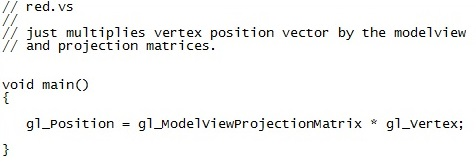
\includegraphics[keepaspectratio=true,scale=1.0]{figuras/red_vs.jpg}
	\caption{\textit{Red vertex shader}}
	\label{red_vs}
	\end{figure}

	Já o seu \textit{fragment shader} estabele que todo fragmento possui a cor vermelha, como é mostrado na Fig. \ref{red_fs}.
	
	
	\begin{figure}[h]
	\centering
		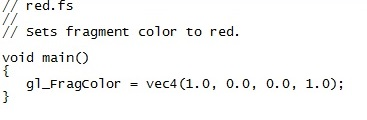
\includegraphics[keepaspectratio=true,scale=1.0]{figuras/red_fs.jpg}
	\caption{\textit{Red fragment shader}}
	\label{red_fs}
	\end{figure}

	O resultado da aplicação deste \textit{shader} é mostrado na Fig. \ref{red_shader}, em que a cor das esferas é vermelha e cada uma delas faz distintas movimentações. 

	\begin{figure}[h]
	\centering
		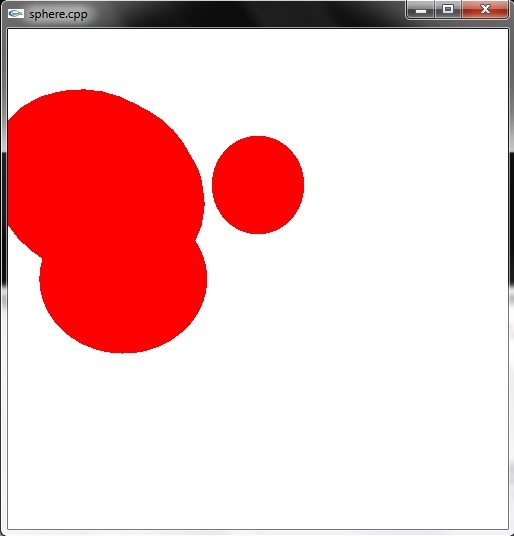
\includegraphics[keepaspectratio=true,scale=0.8]{figuras/red_shader.jpg}
	\caption{\textit{Red shader}}
	\label{red_shader}
	\end{figure}

	\item \textbf{5.1.2 \textit{Flatten shading}}

	A ideia do \textit{flatten shading} é tornar o modelo tridimensional em bidimensional, achatado, e para isso,  a coordenada z deve ser definida como zero. Mas para dar movimentação à malha do objeto, como é mostrado na Fig. \ref{flatten_vs},  foi definida a variável  \textit{time} do tipo \textit{uniform} que é inicializada e passada pelo programa para o \textit{shader}. Assim, a coordenada z varia de acordo de acordo com o fator definido (que inclui esta variável).  

	\begin{figure}[h]
	\centering
		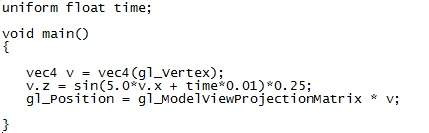
\includegraphics[keepaspectratio=true,scale=1.0]{figuras/flatten_vs.jpg}
	\caption{\textit{Flatten vertex shader}}
	\label{flatten_vs}
	\end{figure}

	Neste caso o \textit{fragment shader} não interfere no resultado desejado e por isso foi utilizado o mesmo do \textit{red shader}, definindo a cor para vermelha. A Fig. \ref{flatten_shader} mostra as esferas achatadas, com a coordenada z variando de acordo com o fator definido. 

	\begin{figure}[h]
	\centering
		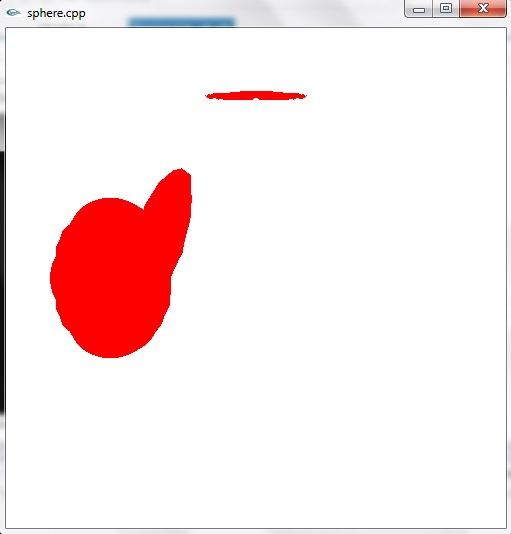
\includegraphics[keepaspectratio=true,scale=0.8]{figuras/flatten_shader.jpg}
	\caption{\textit{Flatten shader}}
	\label{flatten_shader}
	\end{figure}

	\item \textbf{5.1.3 \textit{Toon shading}}

	O  \textit{toon shading} calcula a intensidade da luz por vértice para escolher uma das quatro cores definidas. A Fig. \ref{toon_vs} mostra o cálculo da intensidade da luz por vértice, pegando primeiro a direção da luz (definida como uma variável \textit{uniform} passada pelo programa) para depois fazer o produto escalar entre ela e a normal (adquirida através do comando \textit{gl\_Normal}).  

	\begin{figure}[h]
	\centering
		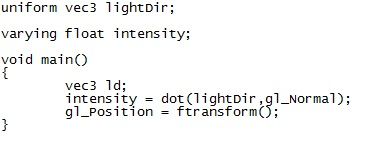
\includegraphics[keepaspectratio=true,scale=0.8]{figuras/toon_vs.jpg}
	\caption{\textit{Toon vertex shader}}
	\label{toon_vs}
	\end{figure}

	A variável \textit{intensity} do tipo \textit{varying} é passada do \textit{vertex shader} para o \textit{fragment shader} - em que como mostra a  Fig. \ref{toon_fs} - para determinar qual das quatro cores será escolhida. 
  
	\begin{figure}[h]
	\centering
		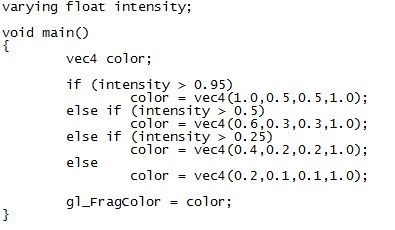
\includegraphics[keepaspectratio=true,scale=0.8]{figuras/toon_fs.jpg}
	\caption{\textit{Toon fragment shader}}
	\label{toon_fs}
	\end{figure}

	Assim, a direção da luz passada pelo programa é {0 , 1 , 1} e o resultado da aplicação do \textit{shder} é mostrado na  Fig. \ref{toon_shader}.

	\begin{figure}[h]
	\centering
		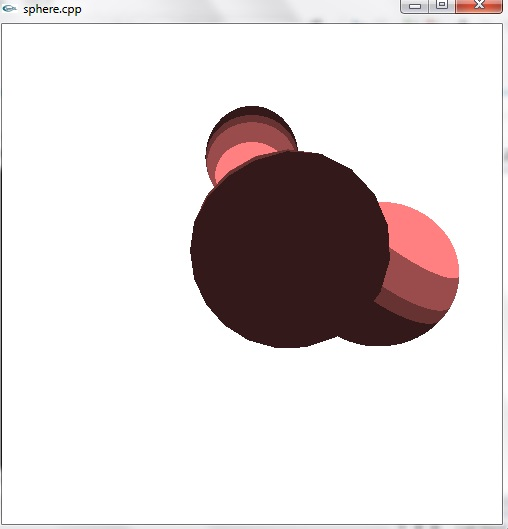
\includegraphics[keepaspectratio=true,scale=0.55]{figuras/toon_shader.jpg}
	\caption{\textit{Toon shader}}
	\label{toon_fs}
	\end{figure}

	\item \textbf{5.1.4 \textit{Phong shading}}

	O \textit{vertex} e \textit{fragment shaders} do \textit{phong shading} implementam a técnica descrita na Seção 2.7. As Fig. \ref{phong_vs} e Fig. \ref{phong_fs} abaixo, mostram as definições do \textit{vertex} e \textit{fragment shaders}, respectivamente, em que para isso é necessário definir as propriedades do material pelo programa.  

	\begin{figure}[h]
	\centering
		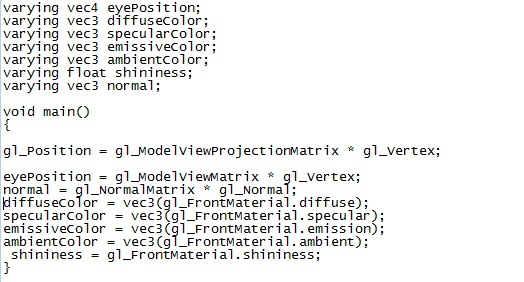
\includegraphics[keepaspectratio=true,scale=1.0]{figuras/phong_vs.jpg}
	\caption{\textit{Phong vertex shader}}
	\label{phong_vs}
	\end{figure}

	\begin{figure}[h]
	\centering
		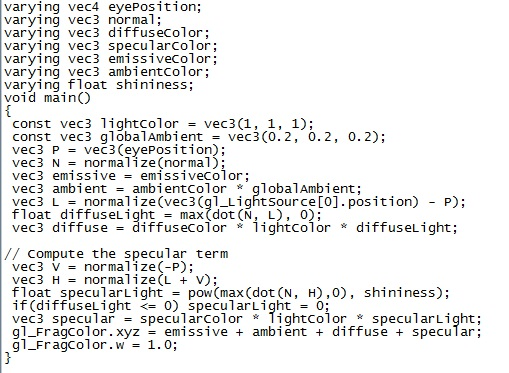
\includegraphics[keepaspectratio=true,scale=1.0]{figuras/phong_fs.jpg}
	\caption{\textit{Phong fragment shader}}
	\label{phong_fs}
	\end{figure}

	O resultado é mostrado na  Fig. \ref{phong_shader}, no qual é muito parecido com o resultado padrão implementado pela  \textit{OpenGL}.

	\begin{figure}[h]
	\centering
		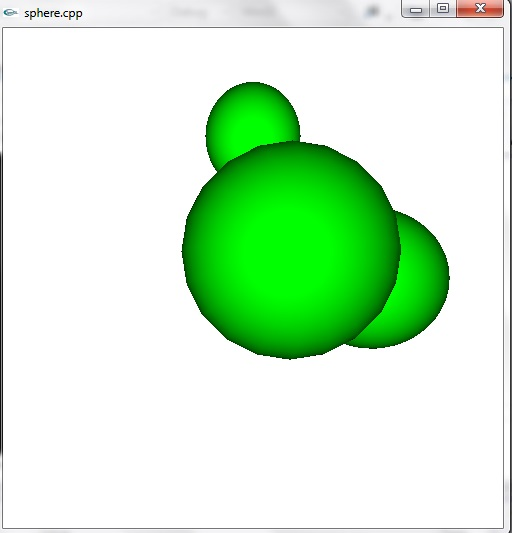
\includegraphics[keepaspectratio=true,scale=0.7]{figuras/phong_shader.jpg}
	\caption{\textit{Phong shader}}
	\label{phong_shader}
	\end{figure}

	\item \textbf{5.1.5 \textit{Texture shading}}

	O \textit{vertex shader} do \textit{texture shading} primeiramente armazena, numa variável do tipo \textit{varying}, as coordenadas da textura por meio do comando \textit{gl\_MultiTexCoord0} para repassar para o \textit{fragment shader}. Vale ressaltar que para este \textit{shader} foi necessário utilizar a função \textit{gluSphere} ao invés da \textit{glutSolidSphere}, pois ela permite especificar um objeto do tipo quádrica, que por sua vez dá opção de criar coordenadas de textura para quádricas (utilizadas pelo \textit{shader}).  

	\begin{figure}[h]
	\centering
		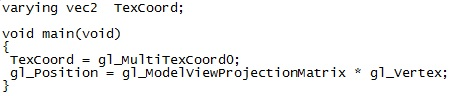
\includegraphics[keepaspectratio=true,scale=1.0]{figuras/texture_vs.jpg}
	\caption{\textit{Texture vertex shader}}
	\label{texture_vs}
	\end{figure}

	O \textit{fragment shader} por sua vez, utiliza a textura da  Fig. \ref{tex} passada pelo programa e aplica na coordenada repassada pelo  \textit{vertex shader}, como mostra a  Fig. \ref{texture_fs}. Assim, o resultado é mostrado na  Fig. \ref{texture_shader}.

	\begin{figure}[h]
	\centering
		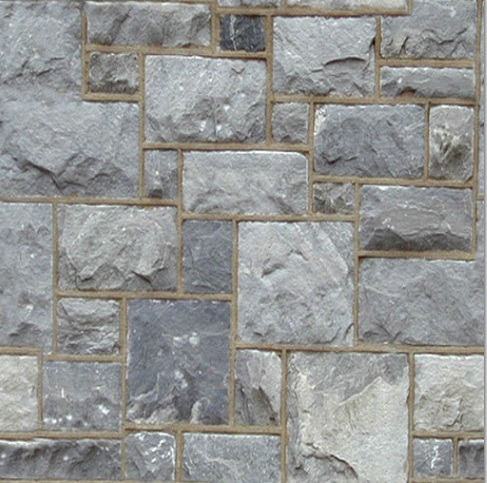
\includegraphics[keepaspectratio=true,scale=0.5]{figuras/tex.jpg}
	\caption{Textura utilizada}
	\label{tex}
	\end{figure}

	\begin{figure}[h]
	\centering
		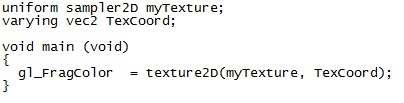
\includegraphics[keepaspectratio=true,scale=1.0]{figuras/texture_fs.jpg}
	\caption{\textit{Fragment shader}}
	\label{texture_fs}
	\end{figure}

	\begin{figure}[h]
	\centering
		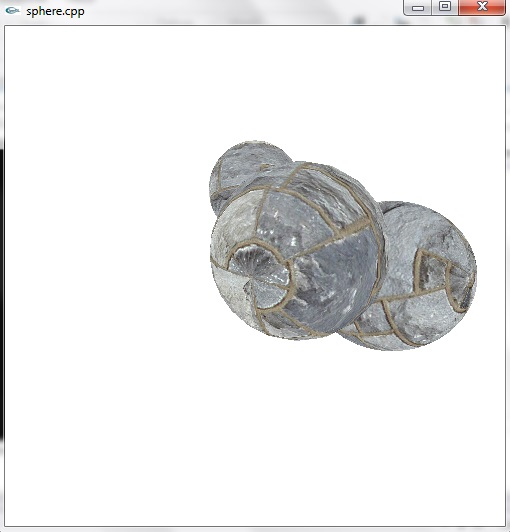
\includegraphics[keepaspectratio=true,scale=0.5]{figuras/texture.jpg}
	\caption{\textit{Texture shader}}
	\label{texture_shader}
	\end{figure}


\end{description}

\section{Gráficos e Análise de Complexidade Algorítmica}

	Após a implementação dos \textit{shaders}, foi utilizada a ferramenta \textit{gDEBugger} descrita na Seção 2.8.2 para fazer medições quanto ao número de quadros por segundo, medida escolhida a fim de avaliar o desempenho, para n números de polígonos. Essa medida de desempenho foi adotada para poder avaliar experimentalmente as complexidades algorítmicas dos \textit{shaders} através das curvas plotadas.

	 A   Fig. \ref{gdebugger} mostra essa ferramenta sendo utilizada, na qual executa-se o programa e a métrica desejada é mostrada em tempo de execução e também pode ser pode ser exportada no formato  \textit{Comma-Separated Values}.  

	\begin{figure}[h]
	\centering
		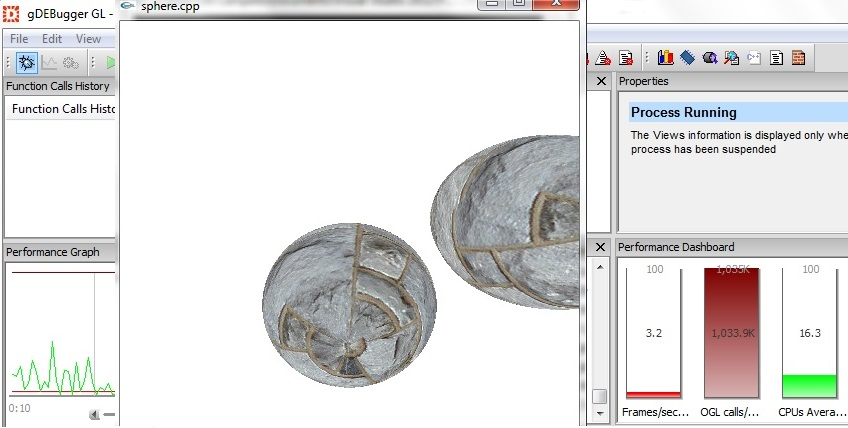
\includegraphics[keepaspectratio=true,scale=0.8]{figuras/gdebugger.jpg}
	\caption{Ferramenta \textit{gDEBugger} sendo utilizada}
	\label{gdebugger}
	\end{figure}

	 Para cada número de subdivisões (no qual foi utilizado o mesmo valor para as subdivisões de latitude e longitude) coletaram-se dez medições, fazendo-se então a média aritmética. O número total de polígonos é dado pela Eq. 
(\ref{eqn00}), em que y é o número de polígonos, sub é o número de subdivisões e esf é a quantidade de esferas. Ao final multiplica-se por dois, pois as subdiviões geram quadriláteros e multiplicando por dois contabilizam-se o número de triângulos (que é o desejado).

	\begin{equation}
	\label{eqn00}
		\mathcal{Y} = sub^{2} \cdot esf \cdot 2
	\end{equation}

	Assim, as medições foram realizadas, para cada \textit{shader} implementado ( \textit{Red, Flatten, Toon, Phong} e  \textit{Texture}). Além disso, variou-se o número de subdivisões das esferas, começando a partir de 50 e incrementando de 25 em 25 até o máximo de subdivisões possíveis, que no caso da esfera utilizada de raio 10, foi de 250. Após este valor, não é possível subdividir mais utilizando as funções da bilblioteca \textit{Glut}. As Tab. (\ref{tab01}), Tab. (\ref{tab02}), Tab. (\ref{tab03}), Tab. (\ref{tab04}), Tab. (\ref{tab05}) abaixo mostram essas medições, evidenciando a quantidade de quadros pro segundo para determinado número de polígonos.  Estas tabelas foram criadas a fim de poder, posteriormente, plotar os gráficos desejados para a análise de complexidade. 

\begin{table}[h]
	\centering
	\begin{tabular}{cccc}
		\toprule
		\textbf{Nº de subdivisões} & \textbf{Nº de polígonos} 
		& \textbf{Quadros/Segundo} & \textbf{Quadros/Segundo} \\
		\midrule
		50 & 15000 & 95.2 & 95.4 \\
		75 & 33750 & 49.6  & 47.1\\
		100 & 60000 & 28.6 & 26.3 \\
		125 & 93750 & 18.8  & 18.3 \\
		150 & 135000 & 13.1 & 12.7 \\
		175 & 183750 & 9.6 & 9.4 \\
		200 & 240000 & 7.4 & 7.1 \\
		225 & 303750 & 6.0 & 5.9 \\
		250 & 375000 & 5.2 & 4.9 \\
		\bottomrule
	\end{tabular}
	\caption{ \textit{Red Shader} e \textit{Flatten Shader}, respectivamente}
	\label{tab01}
\end{table}

\begin{table}[h]
	\centering	
	\begin{tabular}{cccc}
		\toprule
		\textbf{Nº de subdivisões} & \textbf{Nº de polígonos} & 
		\textbf{Quadros/Segundo} & \textbf{Quadros/Segundo}  \\
		\midrule
		50 & 15000 & 95.2  & 96.6\\
		75 & 33750 & 48.8  & 49.3\\
		100 & 60000 &  28.3 & 28.6\\
		125 & 93750 & 18.1 & 18.4\\
		150 & 135000 &  12.9 & 13.1\\
		175 & 183750 &  9.6 & 9.7\\
		200 & 240000 &  7.5 & 7.4\\
		225 & 303750 &  5.9 & 5.8\\
		250 & 375000 &  5.2 & 5.2\\
		\bottomrule
	\end{tabular}
	\caption{ \textit{Toon Shader} e \textit{Phong Shader}, respectivamente}
	\label{tab02}
\end{table}

\begin{table}[h]
	\centering
	\begin{tabular}{ccc}
		\toprule
		\textbf{Nº de subdivisões} & \textbf{Nº de polígonos} & 
		\textbf{Quadros/Segundo}  \\
		\midrule
		50 & 15000 & 76.9  \\
		75 & 33750 & 33.4  \\
		100 & 60000 &  20.3\\
		125 & 93750 & 13.1\\
		150 & 135000 &  9.2\\
		175 & 183750 &  6.8\\
		200 & 240000 &  5.2\\
		225 & 303750 &  4.1\\
		250 & 375000 &  3.4\\
		\bottomrule
	\end{tabular}
	\caption{ \textit{Texture Shader}}
	\label{tab03}
\end{table}

	Com estes dados foi possível traçar as curvas de complexidade algorítmica relativas a cada \textit{texture shader} implementado, tomando como base a quantidade de quadros por segundo. Assim, todas elas foram plotadas em um único gráfico, como é possível ver na Fig. \ref{complexidade}, aparentam a forma de uma função exponencial decrescente. E com exceção da curva do   \textit{texture shader} - que requer maior poder de processamento - as curvas dos outros \textit{shaders} ficaram muito próximas, tanto que no gráfico algumas delas não é possível enxergar. 

	 \begin{figure}[h]
	\centering
		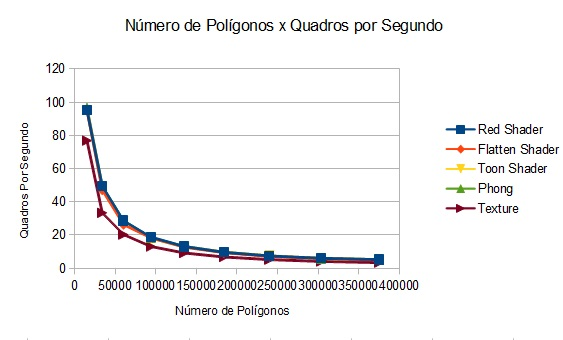
\includegraphics[keepaspectratio=true,scale=1.0]{figuras/complexidade_exp.jpg}
	\caption{Complexidade algoritma: exponencial}
	\label{complexidade}
	\end{figure}

	De acordo com \cite{calculo}, a função da exponencial pode ser dada como na Eq. 
(\ref{eqn01}), em que e, c, k são constantes (e  é a constante neperiana).  

	\begin{equation}
	\label{eqn01}
		y = ce^{-kt}
	\end{equation}

	Aplicando a função logarítimo dos dois lados da equação, obtém-se a  Eq. 
(\ref{eqn02}).

	\begin{equation}
	\label{eqn02}
		\ln{y} = \ln{c}  + \ln{e^{-kt}}
	\end{equation}
 
	Que pode ser simplificada na  Eq. 
(\ref{eqn03}), em que b é uma nova constante, e de acordo com (REFERENCIAR) equivale à equação da reta. 

	\begin{equation}
	\label{eqn03}
		y = b  - kt
	\end{equation}	

	Assim, para confirmar experimentalmente se a  curva obtida dos gráficos é realmente uma exponencial, traçaram-se os gráficos novamente na Fig. \ref{complexidade_reta}, mas dessa vez, na escala logarítmica. 

	\begin{figure}[h]
	\centering
		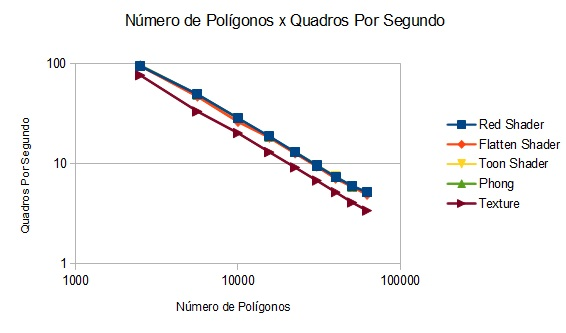
\includegraphics[keepaspectratio=true,scale=1.0]{figuras/complexidade_reta.jpg}
	\caption{\textit{Complexidade Algorítmica: reta}}
	\label{complexidade_reta}
	\end{figure}

	Analisando-se os gráficos, é possível perceber que todos eles se assemelham à uma reta, confirmando as suspeitas levantadas de que a complexidade algorítmica é na ordem exponencial.

\section{Implementação Plataforma \textit{Android}} 

	Para analisar a dificuldade de se implementar na plataforma \textit{Android}, codificou-se o \textit{Gouraud shader} descrito na Seção 2.7, que utiliza a biblioteca \textit{OpenGL ES} e a linguagem de programação Java. Então o programa lê um arquivo obj (descrito na Seção 2.4.4) e renderiza o modelo tridimensional utilizando a técnica de \textit{Vertex Buffer Object} descrita na Seção 2.2.3 e o \textit{shader} mencionado. O resultado se encontra na  Fig. \ref{android}.

	\begin{figure}[h]
	\centering
		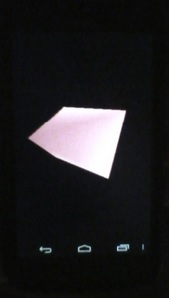
\includegraphics[keepaspectratio=true,scale=1.0]{figuras/android.jpg}
	\caption{Implementação plataforma \textit{Android}}
	\label{android}
	\end{figure}

	Assim, verificou-se que é possível implementar para a plataforma \textit{Android} dentro do prazo estipulado.  

\section{Implementação Computador}

	A fim de se ter uma comparação com o computador, já que a complexidade algorítmica não muda, codificou-se o mesmo programa mostrado na Fig. \ref{computador} , porém utilizando a biblioteca OpenGL, Glut e a linguagem de programa C++.

	\begin{figure}[h]
	\centering
		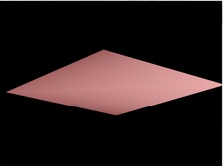
\includegraphics[keepaspectratio=true,scale=1.0]{figuras/computador.jpg}
	\caption{Implementação Computador}
	\label{computador}
	\end{figure}

\section{Conclusão}

	Através dos experimentos realizados foi possível verificar que é factível desenvolver \textit{shaders} para a plataforma \textit{Android} dentro do prazo estipulado. E por meio da plotagem dos gráficos, a ideia de analisar a complexidade algorítmica experimentalmente foi plausível, já que foi obtida uma curva exponencial. Assim, futuramente mais \textit{shaders} poderão ser analisados e implementados tanto para computador quanto para \textit{Android}, utilizando modelos tridimensionais mais complexos, por meio da leitura do arquivo obj. E além disso, com base nas equações extraídas das curvas, o método dos mínimos quadrados - descrito na Seção 2.10 - será utilizado para estimar a  quantidade de quadros por segundo dado um número de polígonos. 
	
	Outro ponto importante a que chegou-se foi com relação entre as diferenças da  \textit{OpenGL} e a  \textit{OpenGL ES}, enquanto convertia-se o mesmo programa para computador.   O principal aspecto notado foi com relação à remoção das chamadas \textit{glBegin} e \textit{glEnd} para desenhar primitivas gráficas e a não utilização do \textit{pipeline} convencional a partir da versão 2.0, em que faz-se obrigatória a utilização de \textit{shaders} pela \textit{OpenGL ES}. Além disso, todo o controle de matrizes de projeção, modelagem (operações de translação, rotação e escalar, por exemplo) e visualização fica a cargo do programador e não mais da \textit{OpenGL ES}. 




